\documentclass[11pt]{article}
\usepackage{minted, tikz}
\usepackage{amsfonts, amssymb, amsmath, float}
\usepackage{enumerate, esint, nicefrac, algorithm2e}
\parindent 0px
\date{February 12, 2024}
\title{CS 401 :\hspace{2px}: Homework 2}
\author{Ryan Magdaleno}

% Helpful ::
% \line(1,0){358px}

\begin{document}
\maketitle

%%%%%%%%%%%%%%%%%%%%%%%%%%%%%%%%%%%%%%%%%%%%%%%%%%%%%%%%%%%%%%%%%%%%%%%%%%%%%%%%%%%%%%%%%

\textbf{Problem 1: Vertex-weighted shortest paths.} 
Let $G = (V, E)$ be an undirected graph and let $w : V\rightarrow\mathbb{R}_{\ge 0}$
be a function that assigns non-negative weights to the vertices of $G$. We define
the \textit{weight} of a path $P=v_1,...,v_k$, denoted by weight$(P)$, to be the
sum of the weights of the vertices in $P$; that is
$$\text{weight}(P)=\sum_{i=1}^k w(v_i).$$
Let $s,t\in V.$ Design a polynomial-time algorithm that computes a path from $s$
to $t$ of minimum weight, if one exists. Show that your algorithm is correct and
that is runs in polynomial time. \\
\vspace{5px}\textbf{Solution ::}

Because this problem deals with an undirected graph with non-negative weights, we can
use a graph algorithm that already exists such as Dijkstra's Algorithm. An issue
however is that Dijkstra's Algorithm only works with non-negative edge weights, not
vertex weights like in this problem. Therefore I'd like to modify the problem a little
to fit Dijkstra's Algorithm. 

\vspace{5px}In a typical implementation of DA (will be calling 
Dijkstra's Algorithm this now) we use a priority queue where each element is the
tentative distances from the source like vertex $s$ in this problem. I'd like each
element in the priority queue to now represent the vertex along with its cumulative
weight from the source $s$.

\vspace{5px}In a typical DA implementation we have some distances container that
keeps track of all cumulative edge weights, we will now use the vertex weights.
Using this we can now compute the tentative distances based on said vertex weights
and update them as the algorithm progresses through the graph.

\pagebreak
Distance container updates are now simply the cumulative weight of the path from
the source vertex $s$ to the current vertex $u$. Updating a neighboring vertex
$v$'s distance if the following condition is met:
$$dist(u) + w(v) < dist(v)$$
where $w(v)$ is the weight of vertex $v$.

\vspace{5px}The algorithm terminates when vertex $t$ is dequeued from the priority
queue, which means we have found a shortest path. If the graph is explored without
ever finding $t$ this indicates there is no connecting path from $s$ to $t$.

\vspace{5px}From this we can reconstruct the minimum-weight $P$ from $s$ to $t$
using a predecessor array, where $prev(u)$ returns the previous vertex on $P$.

\vspace{10px}Algorithm $MinP(G, V, s, t)$:
\begin{algorithm}
    Initialize priority queue $PQ$; \\
    $pred \gets$ array of size $|V|$; \\
    $dist \gets$ array of size $|V|$; \\
    \ForEach{$v \in V$}{
        $dist(v) \gets \infty$; \\
        $pred(v) \gets$ empty; \\
        $PQ$.enqueue($v, \infty$);
    }
    $dist(s)\gets 0$; \\
    $PQ$.enqueue($s,0$); \\
    \While{$PQ$ is not empty}{
        $u, weight_u\gets$ $PQ$.dequeue(); \\
        \If{u = t}{
            \Return{BuildP(pred, s, t);} \\
        }
        \ForEach{neighbor vertex $v$ of $u$}{
            \If{$weight_u + w(v) < dist(v)$} {
                $dist(v)\gets weight_u + w(v)$; \\
                $pred(v)\gets u$; \\
                $PQ$.enqueue$(v, weight_u + w(v))$; 
            }
        }
    }
    \Return{"$s$ and $t$ are not connected in $G$.";}
\end{algorithm}

\pagebreak
\textbf{Polynomial-Time Complexity Proof ::}

Given that $n = |V|=$ the number of vertices in $G$ and $m = |E| =$ is the number of edges
in $G$, if we use a binary heap for our priority queue, we can be sure that our
modified DA implementation is:
$$O((n+m)\cdot\log n)$$

Initializing the predecessor array, distance array, and priority queue all take linear
time, which in this case is:
$$O(n + m)$$
The main while loop in our modified DA implementation iterates at most once for each
vertex in the graph, resulting in:
$$O(n + m)$$
The enqueue, dequeue, and distance updates if implemented with efficient data structures
such as a binary heap will result in:
$$O(\log n)$$
Path reconstruction is also linear in $n$ time, the worst case being a single path through
every vertex resulting in a time complexity of:
$$O(n + m)$$
If we are to combine all these terms together, keeping in mind the inner loop, we come
to a time complexity of:
$$O((n+m)\cdot\log n)$$
This time complexity is indeed polynomial time.
\pagebreak

%%%%%%%%%%%%%%%%%%%%%%%%%%%%%%%%%%%%%%%%%%%%%%%%%%%%%%%%%%%%%%%%%%%%%%%%%%%%%%%%%%%%%%%%%

\textbf{Problem 2: Robot navigation.} Consider a robot that moves inside a room,
represented by a 2-dimensional $n\times n$ square grid. Every location of the grid is indexed by a pair of integers $(i, j)$, where $i, j \in \{1,...,n\}$. Location $(i, j)$
may either be empty, or it might contain an obstacle. The robot is allowed to move only
in empty locations. Apart from its position, the state of the robot also consists of
its orientation, which can be either North, South, West, or East. At every step, the
robot can either move by one position forward in its current orientation, or it
can change its orientation by 90$^{\circ}$. \\
Hint: Express the below problems as shortest-path computations in some graph.
\begin{enumerate}[(a)]
\item
Suppose that initially the robot is positioned at $(1, 1)$ and has orientation North.
The goal is to reach position $(n, n)$ in any orientation. Design an algorithm that 
computes a routing for the robot, with a minimum number of steps. Your algorithm should
run in time polynomial in $n$. \\
\vspace{5px}\textbf{Solution ::} \\
I would like to use an existing algorithm for shortest path traversal, Dijkstra's
Algorithm. This problem however is not able to keep robot orientation in mind. I
would like to construct a graph $G$ which takes orientation in mind with its edges.
For each cell that does not have a obstacle we will create four outgoing edges.
These four edges will all have a weight of 1 each. For example the north orientation
edge will be directed towards the cell $(i, j+1)$, so for cell $(1, 1)$ the northern
edge would be directed towards $(1, 2)$. The robot cannot go into the containing walls
of the grid or into an obstacle so when initially setting up the orientation edges, 
we must not create invalid edges into vertices that are not within the grid or that
contain obstacles.

Each cell will be a vertex, but each of those should become four sub-vertices, making
it so the robot can only move forward one position or change orientation, the four 
sub-vertices will be connected to each other, and they will move towards another set of 
four sub-vertices representing another cell.

\pagebreak
For example, here's an example of a grid converted with no obstacles, $n=4$.
Due to limitations of my drawing, vertex (1, 1) for example is really four vertices each
connected together, the (1, 1) north sub-vertex will go to vertex (2, 1)'s north sub-vertex, all edges including the ones going to another sub-vertex will have an
edge weight of 1, to allow for DA to find a shortest path keeping orientation in
mind:
\begin{center}
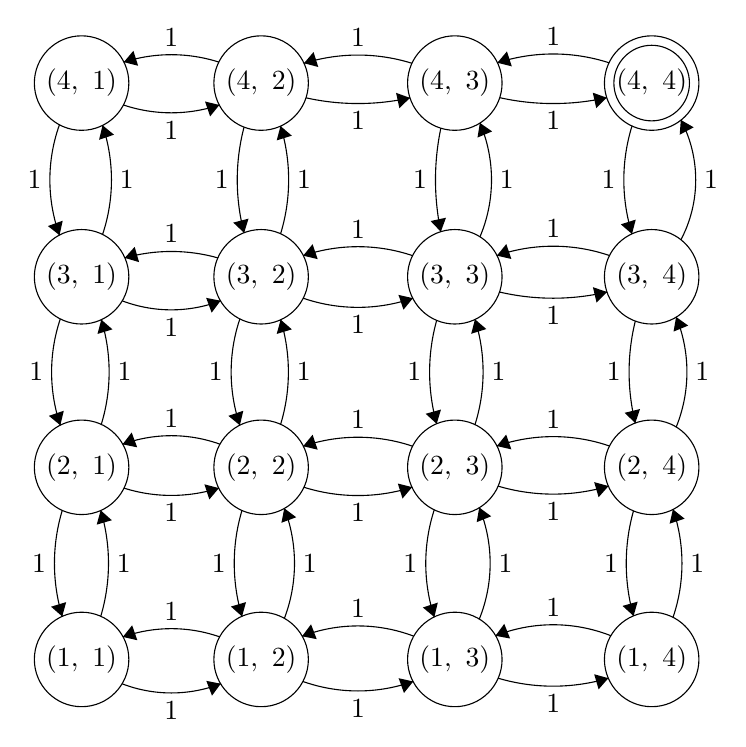
\begin{tikzpicture}[scale=0.2]
\tikzstyle{every node}+=[inner sep=0pt]
\draw [black] (17.5,-45.1) circle (3);
\draw (17.5,-45.1) node {$(1,\mbox{ }1)$};
\draw [black] (28.9,-45.1) circle (3);
\draw (28.9,-45.1) node {$(1,\mbox{ }2)$};
\draw [black] (41.2,-45.1) circle (3);
\draw (41.2,-45.1) node {$(1,\mbox{ }3)$};
\draw [black] (53.7,-45.1) circle (3);
\draw (53.7,-45.1) node {$(1,\mbox{ }4)$};
\draw [black] (17.5,-32.9) circle (3);
\draw (17.5,-32.9) node {$(2,\mbox{ }1)$};
\draw [black] (17.5,-20.8) circle (3);
\draw (17.5,-20.8) node {$(3,\mbox{ }1)$};
\draw [black] (17.5,-8.5) circle (3);
\draw (17.5,-8.5) node {$(4,\mbox{ }1)$};
\draw [black] (28.9,-32.9) circle (3);
\draw (28.9,-32.9) node {$(2,\mbox{ }2)$};
\draw [black] (41.2,-32.9) circle (3);
\draw (41.2,-32.9) node {$(2,\mbox{ }3)$};
\draw [black] (53.7,-32.9) circle (3);
\draw (53.7,-32.9) node {$(2,\mbox{ }4)$};
\draw [black] (28.9,-20.8) circle (3);
\draw (28.9,-20.8) node {$(3,\mbox{ }2)$};
\draw [black] (41.2,-20.8) circle (3);
\draw (41.2,-20.8) node {$(3,\mbox{ }3)$};
\draw [black] (53.7,-20.8) circle (3);
\draw (53.7,-20.8) node {$(3,\mbox{ }4)$};
\draw [black] (28.9,-8.5) circle (3);
\draw (28.9,-8.5) node {$(4,\mbox{ }2)$};
\draw [black] (41.2,-8.5) circle (3);
\draw (41.2,-8.5) node {$(4,\mbox{ }3)$};
\draw [black] (53.7,-8.5) circle (3);
\draw (53.7,-8.5) node {$(4,\mbox{ }4)$};
\draw [black] (53.7,-8.5) circle (2.4);
\draw [black] (18.715,-35.634) arc (16.63983:-16.63983:11.754);
\fill [black] (18.71,-35.63) -- (18.46,-36.54) -- (19.42,-36.26);
\draw (19.71,-39) node [right] {$1$};
\draw [black] (16.274,-42.371) arc (-163.17937:-196.82063:11.65);
\fill [black] (16.27,-42.37) -- (16.52,-41.46) -- (15.56,-41.75);
\draw (15.28,-39) node [left] {$1$};
\draw [black] (18.748,-23.518) arc (17.08548:-17.08548:11.34);
\fill [black] (18.75,-23.52) -- (18.51,-24.43) -- (19.46,-24.14);
\draw (19.75,-26.85) node [right] {$1$};
\draw [black] (16.151,-30.232) arc (-161.31389:-198.68611:10.556);
\fill [black] (16.15,-30.23) -- (16.37,-29.31) -- (15.42,-29.63);
\draw (15.09,-26.85) node [left] {$1$};
\draw [black] (26.332,-22.323) arc (-69.10865:-110.89135:8.784);
\fill [black] (26.33,-22.32) -- (25.41,-22.14) -- (25.76,-23.08);
\draw (23.2,-23.4) node [below] {$1$};
\draw [black] (20.24,-19.602) arc (105.74133:74.25867:10.91);
\fill [black] (20.24,-19.6) -- (21.15,-19.87) -- (20.87,-18.9);
\draw (23.2,-18.69) node [above] {$1$};
\draw [black] (38.536,-22.159) arc (-70.99906:-109.00094:10.708);
\fill [black] (38.54,-22.16) -- (37.62,-21.95) -- (37.94,-22.89);
\draw (35.05,-23.24) node [below] {$1$};
\draw [black] (50.866,-21.768) arc (-76.86812:-103.13188:15.034);
\fill [black] (50.87,-21.77) -- (49.97,-21.46) -- (50.2,-22.44);
\draw (47.45,-22.66) node [below] {$1$};
\draw [black] (43.872,-19.455) arc (108.92573:71.07427:11.033);
\fill [black] (43.87,-19.46) -- (44.79,-19.67) -- (44.47,-18.72);
\draw (47.45,-18.36) node [above] {$1$};
\draw [black] (31.574,-19.461) arc (108.68627:71.31373:10.85);
\fill [black] (31.57,-19.46) -- (32.49,-19.68) -- (32.17,-18.73);
\draw (35.05,-18.39) node [above] {$1$};
\draw [black] (26.218,-34.218) arc (-72.42437:-107.57563:9.994);
\fill [black] (26.22,-34.22) -- (25.3,-33.98) -- (25.61,-34.94);
\draw (23.2,-35.18) node [below] {$1$};
\draw [black] (20.103,-31.435) arc (109.91636:70.08364:9.093);
\fill [black] (20.1,-31.44) -- (21.03,-31.63) -- (20.68,-30.69);
\draw (23.2,-30.39) node [above] {$1$};
\draw [black] (38.489,-34.164) arc (-72.52074:-107.47926:11.448);
\fill [black] (38.49,-34.16) -- (37.58,-33.93) -- (37.88,-34.88);
\draw (35.05,-35.19) node [below] {$1$};
\draw [black] (31.574,-31.561) arc (108.68627:71.31373:10.85);
\fill [black] (31.57,-31.56) -- (32.49,-31.78) -- (32.17,-30.83);
\draw (35.05,-30.49) node [above] {$1$};
\draw [black] (50.956,-34.093) arc (-73.47241:-106.52759:12.323);
\fill [black] (50.96,-34.09) -- (50.05,-33.84) -- (50.33,-34.8);
\draw (47.45,-35.1) node [below] {$1$};
\draw [black] (43.869,-31.55) arc (109.01975:70.98025:10.99);
\fill [black] (43.87,-31.55) -- (44.79,-31.76) -- (44.46,-30.82);
\draw (47.45,-30.45) node [above] {$1$};
\draw [black] (26.343,-46.64) arc (-68.81502:-111.18498:8.697);
\fill [black] (26.34,-46.64) -- (25.42,-46.46) -- (25.78,-47.4);
\draw (23.2,-47.73) node [below] {$1$};
\draw [black] (38.556,-46.495) arc (-70.39933:-109.60067:10.451);
\fill [black] (38.56,-46.5) -- (37.63,-46.29) -- (37.97,-47.23);
\draw (35.05,-47.6) node [below] {$1$};
\draw [black] (50.954,-46.29) arc (-73.52158:-106.47842:12.354);
\fill [black] (50.95,-46.29) -- (50.05,-46.04) -- (50.33,-47);
\draw (47.45,-47.3) node [below] {$1$};
\draw [black] (43.783,-43.596) arc (111.58925:68.41075:9.967);
\fill [black] (43.78,-43.6) -- (44.71,-43.77) -- (44.34,-42.84);
\draw (47.45,-42.4) node [above] {$1$};
\draw [black] (31.5,-43.626) arc (110.90245:69.09755:9.95);
\fill [black] (31.5,-43.63) -- (32.43,-43.81) -- (32.07,-42.87);
\draw (35.05,-42.47) node [above] {$1$};
\draw [black] (20.123,-43.67) arc (109.34289:70.65711:9.291);
\fill [black] (20.12,-43.67) -- (21.04,-43.88) -- (20.71,-42.93);
\draw (23.2,-42.65) node [above] {$1$};
\draw [black] (30.375,-35.499) arc (20.836:-20.836:9.842);
\fill [black] (30.37,-35.5) -- (30.19,-36.42) -- (31.13,-36.07);
\draw (31.52,-39) node [right] {$1$};
\draw [black] (42.75,-35.454) arc (22.12416:-22.12416:9.416);
\fill [black] (42.75,-35.45) -- (42.59,-36.38) -- (43.51,-36.01);
\draw (43.94,-39) node [right] {$1$};
\draw [black] (55.054,-35.566) arc (18.83493:-18.83493:10.636);
\fill [black] (55.05,-35.57) -- (54.84,-36.48) -- (55.79,-36.16);
\draw (56.12,-39) node [right] {$1$};
\draw [black] (52.546,-42.339) arc (-164.28909:-195.71091:12.33);
\fill [black] (52.55,-42.34) -- (52.81,-41.43) -- (51.85,-41.7);
\draw (51.59,-39) node [left] {$1$};
\draw [black] (39.896,-42.409) arc (-161.95463:-198.04537:11.004);
\fill [black] (39.9,-42.41) -- (40.12,-41.49) -- (39.17,-41.8);
\draw (38.85,-39) node [left] {$1$};
\draw [black] (27.685,-42.366) arc (-163.36017:-196.63983:11.754);
\fill [black] (27.69,-42.37) -- (27.94,-41.46) -- (26.98,-41.74);
\draw (26.69,-39) node [left] {$1$};
\draw [black] (30.137,-23.524) arc (16.91222:-16.91222:11.435);
\fill [black] (30.14,-23.52) -- (29.89,-24.43) -- (30.85,-24.14);
\draw (31.13,-26.85) node [right] {$1$};
\draw [black] (30.135,-11.225) arc (17.0251:-17.0251:11.697);
\fill [black] (30.13,-11.23) -- (29.89,-12.14) -- (30.85,-11.84);
\draw (31.15,-14.65) node [right] {$1$};
\draw [black] (42.478,-23.504) arc (17.55762:-17.55762:11.092);
\fill [black] (42.48,-23.5) -- (42.24,-24.42) -- (43.2,-24.12);
\draw (43.5,-26.85) node [right] {$1$};
\draw [black] (42.793,-11.027) arc (22.97075:-22.97075:9.284);
\fill [black] (42.79,-11.03) -- (42.64,-11.96) -- (43.57,-11.57);
\draw (44.03,-14.65) node [right] {$1$};
\draw [black] (55.255,-23.35) arc (22.12105:-22.12105:9.293);
\fill [black] (55.25,-23.35) -- (55.09,-24.28) -- (56.02,-23.9);
\draw (56.44,-26.85) node [right] {$1$};
\draw [black] (55.552,-10.839) arc (27.83915:-27.83915:8.161);
\fill [black] (55.55,-10.84) -- (55.48,-11.78) -- (56.37,-11.31);
\draw (57,-14.65) node [right] {$1$};
\draw [black] (27.817,-18.009) arc (-165.29497:-194.70503:13.233);
\fill [black] (27.82,-18.01) -- (28.1,-17.11) -- (27.13,-17.36);
\draw (26.88,-14.65) node [left] {$1$};
\draw [black] (27.552,-30.231) arc (-161.34301:-198.65699:10.569);
\fill [black] (27.55,-30.23) -- (27.77,-29.31) -- (26.82,-29.63);
\draw (26.5,-26.85) node [left] {$1$};
\draw [black] (40.049,-30.138) arc (-164.40886:-195.59114:12.232);
\fill [black] (40.05,-30.14) -- (40.32,-29.23) -- (39.35,-29.5);
\draw (39.1,-26.85) node [left] {$1$};
\draw [black] (52.662,-30.092) arc (-166.0879:-193.9121:13.484);
\fill [black] (52.66,-30.09) -- (52.96,-29.2) -- (51.98,-29.44);
\draw (51.77,-26.85) node [left] {$1$};
\draw [black] (52.452,-18.081) arc (-162.76875:-197.23125:11.582);
\fill [black] (52.45,-18.08) -- (52.69,-17.17) -- (51.74,-17.47);
\draw (51.43,-14.65) node [left] {$1$};
\draw [black] (40.313,-17.939) arc (-168.14746:-191.85254:16.012);
\fill [black] (40.31,-17.94) -- (40.64,-17.05) -- (39.66,-17.26);
\draw (39.47,-14.65) node [left] {$1$};
\draw [black] (16.096,-18.16) arc (-160.2617:-199.7383:10.395);
\fill [black] (16.1,-18.16) -- (16.3,-17.24) -- (15.36,-17.58);
\draw (14.99,-14.65) node [left] {$1$};
\draw [black] (18.83,-11.178) arc (18.53816:-18.53816:10.919);
\fill [black] (18.83,-11.18) -- (18.61,-12.1) -- (19.56,-11.78);
\draw (19.9,-14.65) node [right] {$1$};
\draw [black] (26.254,-9.887) arc (-71.33924:-108.66076:9.545);
\fill [black] (26.25,-9.89) -- (25.34,-9.67) -- (25.66,-10.62);
\draw (23.2,-10.89) node [below] {$1$};
\draw [black] (38.355,-9.436) arc (-77.43851:-102.56149:15.196);
\fill [black] (38.35,-9.44) -- (37.47,-9.12) -- (37.68,-10.1);
\draw (35.05,-10.3) node [below] {$1$};
\draw [black] (50.852,-9.427) arc (-77.45934:-102.54066:15.666);
\fill [black] (50.85,-9.43) -- (49.96,-9.11) -- (50.18,-10.09);
\draw (47.45,-10.3) node [below] {$1$};
\draw [black] (43.901,-7.214) arc (107.98845:72.01155:11.493);
\fill [black] (43.9,-7.21) -- (44.82,-7.44) -- (44.51,-6.49);
\draw (47.45,-6.15) node [above] {$1$};
\draw [black] (31.615,-7.245) arc (107.34984:72.65016:11.518);
\fill [black] (31.62,-7.24) -- (32.53,-7.48) -- (32.23,-6.53);
\draw (35.05,-6.22) node [above] {$1$};
\draw [black] (20.176,-7.17) arc (107.7535:72.2465:9.916);
\fill [black] (20.18,-7.17) -- (21.09,-7.4) -- (20.79,-6.45);
\draw (23.2,-6.2) node [above] {$1$};
\end{tikzpicture}
\end{center}

\pagebreak
Here's an example with $n = 4$ and obstacles $= \{(2,2), (3,2), (3,3), (3,4)\}$

\begin{center}
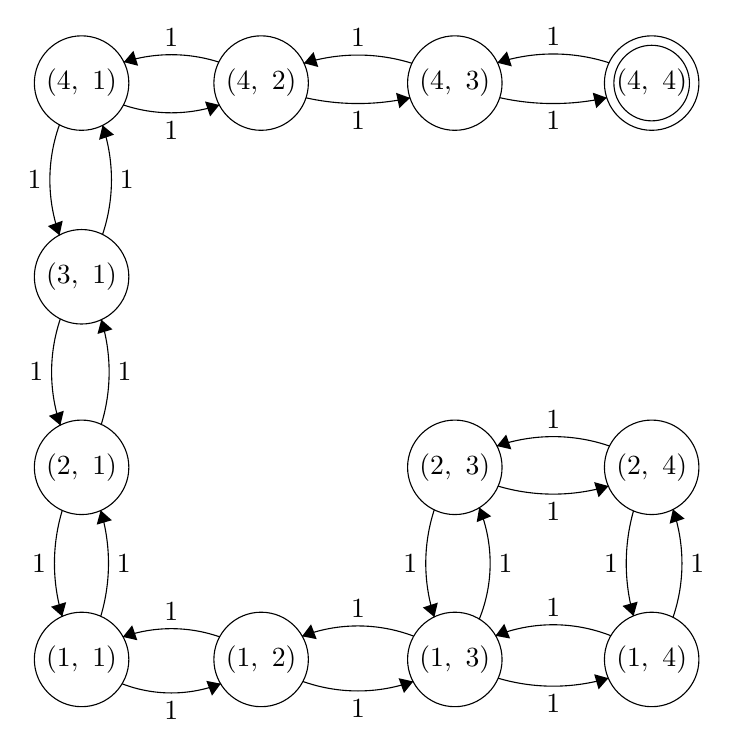
\begin{tikzpicture}[scale=0.2]
\tikzstyle{every node}+=[inner sep=0pt]
\draw [black] (17.5,-45.1) circle (3);
\draw (17.5,-45.1) node {$(1,\mbox{ }1)$};
\draw [black] (28.9,-45.1) circle (3);
\draw (28.9,-45.1) node {$(1,\mbox{ }2)$};
\draw [black] (41.2,-45.1) circle (3);
\draw (41.2,-45.1) node {$(1,\mbox{ }3)$};
\draw [black] (53.7,-45.1) circle (3);
\draw (53.7,-45.1) node {$(1,\mbox{ }4)$};
\draw [black] (17.5,-32.9) circle (3);
\draw (17.5,-32.9) node {$(2,\mbox{ }1)$};
\draw [black] (17.5,-20.8) circle (3);
\draw (17.5,-20.8) node {$(3,\mbox{ }1)$};
\draw [black] (17.5,-8.5) circle (3);
\draw (17.5,-8.5) node {$(4,\mbox{ }1)$};
\draw [black] (41.2,-32.9) circle (3);
\draw (41.2,-32.9) node {$(2,\mbox{ }3)$};
\draw [black] (53.7,-32.9) circle (3);
\draw (53.7,-32.9) node {$(2,\mbox{ }4)$};
\draw [black] (28.9,-8.5) circle (3);
\draw (28.9,-8.5) node {$(4,\mbox{ }2)$};
\draw [black] (41.2,-8.5) circle (3);
\draw (41.2,-8.5) node {$(4,\mbox{ }3)$};
\draw [black] (53.7,-8.5) circle (3);
\draw (53.7,-8.5) node {$(4,\mbox{ }4)$};
\draw [black] (53.7,-8.5) circle (2.4);
\draw [black] (18.715,-35.634) arc (16.63983:-16.63983:11.754);
\fill [black] (18.71,-35.63) -- (18.46,-36.54) -- (19.42,-36.26);
\draw (19.71,-39) node [right] {$1$};
\draw [black] (16.274,-42.371) arc (-163.17937:-196.82063:11.65);
\fill [black] (16.27,-42.37) -- (16.52,-41.46) -- (15.56,-41.75);
\draw (15.28,-39) node [left] {$1$};
\draw [black] (18.748,-23.518) arc (17.08548:-17.08548:11.34);
\fill [black] (18.75,-23.52) -- (18.51,-24.43) -- (19.46,-24.14);
\draw (19.75,-26.85) node [right] {$1$};
\draw [black] (16.151,-30.232) arc (-161.31389:-198.68611:10.556);
\fill [black] (16.15,-30.23) -- (16.37,-29.31) -- (15.42,-29.63);
\draw (15.09,-26.85) node [left] {$1$};
\draw [black] (50.956,-34.093) arc (-73.47241:-106.52759:12.323);
\fill [black] (50.96,-34.09) -- (50.05,-33.84) -- (50.33,-34.8);
\draw (47.45,-35.1) node [below] {$1$};
\draw [black] (43.869,-31.55) arc (109.01975:70.98025:10.99);
\fill [black] (43.87,-31.55) -- (44.79,-31.76) -- (44.46,-30.82);
\draw (47.45,-30.45) node [above] {$1$};
\draw [black] (26.343,-46.64) arc (-68.81502:-111.18498:8.697);
\fill [black] (26.34,-46.64) -- (25.42,-46.46) -- (25.78,-47.4);
\draw (23.2,-47.73) node [below] {$1$};
\draw [black] (38.556,-46.495) arc (-70.39933:-109.60067:10.451);
\fill [black] (38.56,-46.5) -- (37.63,-46.29) -- (37.97,-47.23);
\draw (35.05,-47.6) node [below] {$1$};
\draw [black] (50.954,-46.29) arc (-73.52158:-106.47842:12.354);
\fill [black] (50.95,-46.29) -- (50.05,-46.04) -- (50.33,-47);
\draw (47.45,-47.3) node [below] {$1$};
\draw [black] (43.783,-43.596) arc (111.58925:68.41075:9.967);
\fill [black] (43.78,-43.6) -- (44.71,-43.77) -- (44.34,-42.84);
\draw (47.45,-42.4) node [above] {$1$};
\draw [black] (31.5,-43.626) arc (110.90245:69.09755:9.95);
\fill [black] (31.5,-43.63) -- (32.43,-43.81) -- (32.07,-42.87);
\draw (35.05,-42.47) node [above] {$1$};
\draw [black] (20.123,-43.67) arc (109.34289:70.65711:9.291);
\fill [black] (20.12,-43.67) -- (21.04,-43.88) -- (20.71,-42.93);
\draw (23.2,-42.65) node [above] {$1$};
\draw [black] (42.75,-35.454) arc (22.12416:-22.12416:9.416);
\fill [black] (42.75,-35.45) -- (42.59,-36.38) -- (43.51,-36.01);
\draw (43.94,-39) node [right] {$1$};
\draw [black] (55.054,-35.566) arc (18.83493:-18.83493:10.636);
\fill [black] (55.05,-35.57) -- (54.84,-36.48) -- (55.79,-36.16);
\draw (56.12,-39) node [right] {$1$};
\draw [black] (52.546,-42.339) arc (-164.28909:-195.71091:12.33);
\fill [black] (52.55,-42.34) -- (52.81,-41.43) -- (51.85,-41.7);
\draw (51.59,-39) node [left] {$1$};
\draw [black] (39.896,-42.409) arc (-161.95463:-198.04537:11.004);
\fill [black] (39.9,-42.41) -- (40.12,-41.49) -- (39.17,-41.8);
\draw (38.85,-39) node [left] {$1$};
\draw [black] (16.096,-18.16) arc (-160.2617:-199.7383:10.395);
\fill [black] (16.1,-18.16) -- (16.3,-17.24) -- (15.36,-17.58);
\draw (14.99,-14.65) node [left] {$1$};
\draw [black] (18.83,-11.178) arc (18.53816:-18.53816:10.919);
\fill [black] (18.83,-11.18) -- (18.61,-12.1) -- (19.56,-11.78);
\draw (19.9,-14.65) node [right] {$1$};
\draw [black] (26.254,-9.887) arc (-71.33924:-108.66076:9.545);
\fill [black] (26.25,-9.89) -- (25.34,-9.67) -- (25.66,-10.62);
\draw (23.2,-10.89) node [below] {$1$};
\draw [black] (38.355,-9.436) arc (-77.43851:-102.56149:15.196);
\fill [black] (38.35,-9.44) -- (37.47,-9.12) -- (37.68,-10.1);
\draw (35.05,-10.3) node [below] {$1$};
\draw [black] (50.852,-9.427) arc (-77.45934:-102.54066:15.666);
\fill [black] (50.85,-9.43) -- (49.96,-9.11) -- (50.18,-10.09);
\draw (47.45,-10.3) node [below] {$1$};
\draw [black] (43.901,-7.214) arc (107.98845:72.01155:11.493);
\fill [black] (43.9,-7.21) -- (44.82,-7.44) -- (44.51,-6.49);
\draw (47.45,-6.15) node [above] {$1$};
\draw [black] (31.615,-7.245) arc (107.34984:72.65016:11.518);
\fill [black] (31.62,-7.24) -- (32.53,-7.48) -- (32.23,-6.53);
\draw (35.05,-6.22) node [above] {$1$};
\draw [black] (20.176,-7.17) arc (107.7535:72.2465:9.916);
\fill [black] (20.18,-7.17) -- (21.09,-7.4) -- (20.79,-6.45);
\draw (23.2,-6.2) node [above] {$1$};
\end{tikzpicture}
\end{center}

Using Dijkstra's Algorithm the robot should be able to find the shortest path from
$(1,1)$ to $(n,n)$. \pagebreak

Algorithm $Dijkstra\_Plus\_New\_G(obstacles, n)$:
\begin{algorithm}
    Initialize $n\times n\,\, G$; \\
    \ForEach{$o\in obstacles$}{
        removeConnectedEdges($G, o$);
    }
    \,\\
    // Dijkstra's Algorithm from here onwards:\\
    Initialize priority queue $PQ$; \\
    $pred\gets$ array of size $n^2$; \\
    $dist\gets$ array of size $n^2$; \\
    \ForEach{$v\in G$}{
        $dist(v)\gets\infty$; \\
        $pred(v)\gets$ empty; \\
        $PQ$.enqueue($v, \infty$);
    }
    $dist((1, 1))\gets 0;$ \\
    $PQ$.enqueue($(1,1)$, 0); \\
    \While{PQ is not empty}{
        $u, weight_u\gets PQ$.dequeue(); \\
        \If {$u = (n,n)$ }{
            \Return{BuildP(pred, (1,1), (n,n))};
        }
        \ForEach{neighbor edge $e$ of $u$}{
            \If{$weight_u + w(e) < dist(v)$}{
                $dist(e)\gets weight_u + w(e)$; \\
                $pred(e)\gets u;$ \\
                $PQ$.enqueue($e, weight_u + w(e)$);
            }
        }
    }
    \Return{"$(1,1)$ and $(n, n)$ are not connected in $G$.";}
\end{algorithm}
\pagebreak

\textbf{Polynomial-Time Complexity Proof ::} \\
Firstly, we build the $n\times n$ grid graph $G$. For each empty cell,
we check all four directions for if there is a valid cell to create an edge towards.
This results in a $O(n^2)$ time complexity for building the graph $G$.

Assuming the worst case number of vertices and edges we get $|V| = n^2$,
$|E| = 4 n^2$. Dijkstra's Algorithm runs in $O((|V| + |E|)\cdot \log |V|)$ time.
The reason for why in the worst case $|V| = n^2$ is that if there are no obstacles we
can have at most $n^2$ vertices in our graph $G$. For edges in the worst case, if there
are no obstacles then no vertices get removed, which means no edges get removed. There
are four directions and in the worst case $|E| = 4n^2$.

Therefore, the time complexity of Dijkstra's Algorithm in this case is:
$$O((n^2 + 4n^2)\cdot\log n^2) = O(n^2\cdot\log n^2)$$

\pagebreak

\item
Suppose that there are $k$ robots in the room. At each step every robot moves 
simultaneously. Two robots cannot occupy the same location and they cannot pass through each other. You are given the starting position and orientation of each robot and its 
destination. Design an algorithm that computes the shortest sequence of steps that move 
all the robots to their respective destinations. The running time of your algorithm should be $n^{O(k)}$. \\
\vspace{5px}\textbf{Solution ::} \\
Let us represent the graph G like in part a, where obstacle vertices are removed and each 
cell is a set of four vertices. This problem however has us control multiple robots. The 
goal is to avoid collisions
during movements. We can run Dijkstra's Algorithm on all robots towards the 
given destination coordinates. We should then check how many robots are on each shortest
path, we should prioritize moving robots with the lowest amount of robots on its path. 
So we should sort the number of encountered robots on each $k_i$ robot's shortest path. 
If it occurs that there is a collision immenent, we will stop one robot for that 
movement, this way it allows for one robot to proceed on its shortest path. After that we 
would run Dijkstra's Algorithm again to check the new shortest path for all robots and 
repeat these steps until the $k$th robot reaches its respective destination.

This is assuming that all robots and their respective destination coordinates are 
connected by atleast one path, if the first Dijkstra's Algorithm search doesn't find
a path, then the robot(s) that couldn't find their path should be removed.

\pagebreak

$dests$ is the coordinates expressed in tuple form $(x, y)$, $x\ge 1$, $y\ge 1$ \\
$obstacles$ is the vertices to remove from $G$. \\
$kRobotPos$ is the current robot positions. \\
Algorithm $kRobotsDijkstra(dests, obstacles, kRobotPos, n, k)$:
\begin{algorithm}
    Initialize $n\times n$ $G$; \\
    $robotPaths \gets$ array of size $k$; \\
    \ForEach{$o\in obstacles$}{
        removeConnectedEdges($G, o$);
    }
    \While{$k > 0$}{
        \ForEach{$robotPos\in kRobotPos$}{
            $dest \gets dests(robotPos)$; \\
            $robotPath\gets Dijkstra(G, robotPos, dest)$; \\
            $robotPaths$.append($robotPath$); \\
        }
        $robotPaths$.sort(); \\
        \ForEach{path in robotPaths}{
            \If{$collision(G, path)$}{
                continue;
            }
            $moveRobotOnPath(G, path);$ \\
            $k\gets k-1;$ 
        }

        %$k\gets k - 1;$
    }




\end{algorithm}

\pagebreak

\textbf{Time Complexity Proof ::}

There are $4n^2 = n^2$ vertices in $G$, there are $8n^2 = n^2$ edges in $G$.
In the worst case, for each cell, there will be 8 edges, 4 for the orientation
vertices and 4 for out going edges to other cells. Therefore construction of graph $G$
takes: $$O(n^2)$$

Because we run Dijkstra's Algorithm on every move we need to first check DA's time
complexity and check the largest amount of moves before the $k$th robot reaches its destination. Dijkstra's Algorithm for this graph takes:
$$O((n^2 + n^2)\cdot\log n^2) = O(n^2\cdot\log n^2)$$

In the worst case the amount of moves is linked to the size of the grid so therefore
the amount of moves is some constant times $n$. There is also a sorting step of
$O(k\cdot\log k)$

Therefore in one move there is: $$O((k\cdot\log k)\cdot k\cdot (n^2\cdot\log n^2))
= O((k^2\cdot \log k)\cdot (n^2\cdot\log n^2))$$

All together if we have an $n\times n$ grid the time complexity would be:
$$n^{O((k^2\cdot \log k)\cdot (n^2\cdot\log n^2))}$$
Where in the worst case, we have some $n$ sized grid and therefore have $n$ amount
of moves, where on each move we must do Dijkstra's algorithm $k$ number of times.

\end{enumerate}

\pagebreak

%%%%%%%%%%%%%%%%%%%%%%%%%%%%%%%%%%%%%%%%%%%%%%%%%%%%%%%%%%%%%%%%%%%%%%%%%%%%%%%%%%%%%%%%%

\textbf{Problem 3: Finding a cheap flight.} Let $G = (V, E)$ be a directed graph, where
$V$ is a set of cities, and $E$ represents all possible flights between the cities in 
$V$. For every edge ${u, v} \in E$, you are given the duration of a direct flight from 
$u$ to $v$, denoted by $d(u, v)$, which is an integer. For example, if you are at city
$u$ at time $t$, and you take a direct flight to $v$, departing at time $t'\ge t$, then 
you arrive at $v$ at time $t' + d(u, v)$. For every $\{u, v\}\in E$, you are given a 
timetable of all available direct flights from $u$ to $v$, for some interval 
$\{0,...,T\}$, where $T > 0$ is an integer. That is, for any $\{u, v\}\in E$, you are
given a list of pairs of integers $((t_u,v,1, c_u,v,1),...,(t_u,v,k, c_u,v,k))$, where 
the pair $(t_u,v,i, c_u,v,i)$ denotes the fact that there is a direct flight from $u$ to
$v$ that departs at time $t_u,v,i$, and costs $c_u,v,i$ dollars. Design an algorithm
that given a pair of cities $u, v\in V$, computes the cheapest possible route
that starts at $u$ at time 0, and ends at $v$ at time at most $T$. The running time of 
your algorithm should be polynomial in $|V|$, and $T$. \\
\vspace{5px}\textbf{Solution ::} \\
This problem is giving us a directed graph $G$ that represents cities as vertices and
flights between cities as edges. We are trying to find the cheapest flight path
from city $u$ to city $v$, and must end at most at time $T$.

\vspace{10px}We will need to keep track of each cities minimum costs at each step of the way. First we need to initialize a container that keeps track of each city's cost
at each time $t_{i}$ up to T, for example cell $(i, j)$ will represent city $i$ at 
time $j$, $0\le j \le T$. We will make this $|V|\times T$ table and call it $R$

\vspace{10px}To start off we must set city $u$ at time 0 like so:
$$\text{R}[u][0]\gets 0$$
For all other cities in $V$ we will set their initial cost to infinity, we are
essentially going to minimize the cost as we traverse the graph.

\vspace{10px}Now we are to go over all times from $0$ to $T$ for each city $u$.
We are to also check for each city $u$, each outgoing flight from $u$ to $v$ at our
current time $t$.

We will update the table on the condition that $t' + d(u, v) \le T$, the new min
cost would become:
$$R[v][t' + d(u, v)]\gets min(R[v][t'+d(u,v)], R[u][t] + c_u)$$

The algorithm would then return the minimum cost from $R[v][T]$ if it's not infinity,
infinity indicates there was not a path to the final destination. This solution constructs
the cheapest paths using the graph, in a sort of greedy manner.

\pagebreak

Algorithm $cheapest(G, T, V, u, v)$:

\begin{algorithm}
    Initialize $R$ $\gets$ container with dimensions $|V|\times T$; \\
    \ForEach{city $u' \in V$}{
        $t\gets 0$; \\
        \While{$t\le T$}{
            $R[u'][t] = \infty$; \\
        }
    }
    Mark start city: $R[u][0]\gets 0$; \\
    $t\gets 0$; \\
    \While{$t\le T$}{
        \ForEach{city $u$}{
            \ForEach{$(t_u, v, i, c_u, v, i)$}{
                \If{$t + d(u, v) \le T$} {
                    $R[v][t + d(u, v)]\gets min(R[v][t + d(u,v)], R[u][t] + c_u)$;
                }
            }
        }
        $t\gets t + 1;$
    }
    \If{$R[v][T] = \infty$}{
        \Return {
            "No route";
        }
    }
    \Else{
        \Return{
            $R[v][T]$;
        }
    }
\end{algorithm}

\pagebreak

\textbf{Time-Complexity Analysis ::}

Initializing the $R$ container takes two nested loops, the outer in $O(|V|)$ time and
the inner loop in $O(T)$ time, all together this is:
$$O(|V|\cdot T)$$

There are three nested loops, the outer loop iterates $t$ from 0 to $T$, therefore this
is: $$O(T)$$

The next loop layer iterates over all cities $u$, the number of cities is $|V|$, therefore
it is: $$O(|V|)$$

The next loop layer iterates over each outgoing flight from $u$, which could have be
$|E|$ if you consider the worst case, therefore it is:
$$O(|E|)$$

Combining our loops we get the following time complexity if you consider the worst case
scenario:
$$O(T\cdot |V|\cdot |E|)$$

This time complexity satisfies the constraint that it must be a polynomial in $|V|$,
and $T$.
\end{document}